\documentclass{article}
\usepackage{graphicx}
\usepackage{fancyhdr}
\pagestyle{fancy}
\lhead{Ruicheng Wu}
\rhead{07/25/2017}
\chead{Homework 11}

\begin{document}
1.

a)

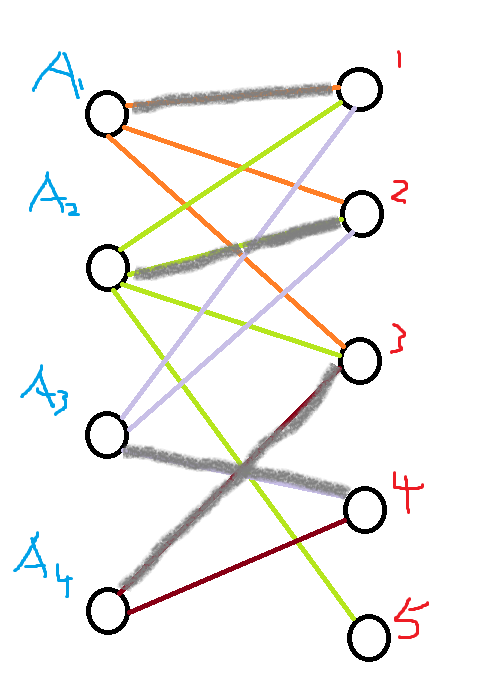
\includegraphics[scale=0.5]{HW11_a.png}

b)

Can not draw a bipartite graph:

Assume subset R = $(A_1 , A_3 , A_4)$, the cardinality is 3 ; and the $\gamma(R)$ = 2 ,because $(A_1 \cap A_3 \cap A_4) = (1,2)$. The Hall's marriage condition fails.

2.

Given $$\gamma_(R)\geq |R| $$

We can know there is a matching of size $|R|$.

Think of adding d vertices to Y that every adding vertices are adjacent to vertices in X. We can know the |R| won't change.

However the new $$\gamma_{new}(R) = \gamma_(R) + d$$

plug into the new equation, we can obtain that $$\gamma_(R) + d \geq |R|$$ $$\gamma_(R) \geq |R| - d$$,so the condition given actually means adding d vertices like i did above.

Now we can substitute $|R| - d$ by $|S|$,we will have$\gamma_(S) \geq |S|$,that is there is a matching of size $|S|$ and thus $|R| - d$.

We know $R \subset X$. So X will apply to this. There exists a matching of size $|X| - d$.

3.

Given there are 5 points in total on a sphere.

Consider there are 2 circles through any 2 of
the points. 

This partitions the sphere into 2 hemispheres. By the pigeonhole principle, 2 of the rest 3 points must lie in one of the hemispheres.

These 2 points, along with the original 2 points, lie in a closed semi-sphere. Thus, the problem is proved.

4.

From Ramsey’s Theorem

$R(n,n) \leq C(2n-2,n-1)$,here since we are asked to prove there must a group of 7 people have two situations : completely stranger or completely know each other, we plug $n = 7$ in. Result in $$R(7,7) \leq C(12,6) = 924$$.

This means 924 attendees is the number can definitely contains such substructure of group of 7 people, and we are given 1000 people. Thus it proves the question.

5.\\

a)
Simply,we talk about $red K_3$  first:

There are two conditions:

\begin{large}
First:
\end{large} 
all 3 vertices ,say A-B-C,are adjacent to each other,then in a 8 vertices "circle" graph, the A and C can never be opposite to each other,so there is never a red edge between A and C. This condition fails.

\begin{large}
Second:
\end{large} 
3 vertices not adjacent to each other(2 or them may be adjacent).From the property of this graph, only opposite vertices will contain red edge,so no matter how we choose the combination for 3 vertices,there must one blue edge coming from the non-opposite one.

There is no red $K_3$ in this case!

Now we consider  $blue K_4$:
If we choose adjacent vertices from the circle,the edges between neighbors are red according to the given graph,so how can it possibly have a $blue K_4$ in this case. 

If we choose any 4 non-adjacent vertices,there $K_4$ must contain opposite pair,so there is red edges.

There is neither blue $K_4$ in this case!

So the union of both cases is no.\\

b)

Given n vertices,a vertex $v$ will have n-1 edges incident on it. Now suppose there are more than 3 red edges(at least 4) or more than 5 blue edges(at 6) incident on it.

Let's discuss about at least 6 blue edges:

Consider the endpoints {$v_1,...,v_6,...v_{n-1}$} of those edges. Among these n-1 vertices, there will be a $K_6$ is coloured red and blue; By Ramsey's Fact 3.2.1, this $K_6$ contains either a red
$K_3$ or a blue $K_3$. A blue $K_3$ among vertices {$v_a
, v_b , v_c$}, together with the blue edges to $v$ from
each of these, will form a blue $K_4$. Thus, if v has at least 6 blue edges(more than 5) incident on it, we are guaranteed there is either a red $K_3$ or a blue $K_4$.\\

c)from b),we know there is at least 4 red edges or at least 6 blue edges to one vertex,then there will be red $K_3$ or a blue $K_4$.
According to the situation of edges,there must be at least 9 edges.
Since it is a $K_n$. $n-1 = 9$ turns out $n = 10$. Then R(3,4) tells us the number of vertices that can make a red $K_3$ or blue $K_4$. Now that number is 10. So we prove $R(3,4) \leq 10$\\

d)Given every vertex has exactly 3 red and 5 blue edges in $K_9$.We know that $K_9$ has total 

\begin{large}
$\frac{(9-1)*9}{2}$= 36 edges
\end{large}

Since every vertex has same rate between red and blue edges which is 3:5;then there will be $\frac{108}{8}$ red edges and $\frac{180}{8}$ blue edges which is not possible.

Hence we prove the only possibility that $K_9$ has neither a red $K_3$ nor a blue $K_4$ is not possible.\\

e)From c), we already exclude the situation that every vertex has exactly 3 red and 5 blue edges in $K_9$ is impossible.So there are all other different pairs existing (1R7B,2R6B,3R5B,4R4B,5R3B,6R2B,7R1B)among all vertices. Just all of them can not be all in one pattern.Then there will exist one pair that satisfy the condition at least 4R or at least 6B . So $K_9$ also satisfy R(3,4). 

Then we can conclude that $$R(3,4) \leq 9$$
 

\end{document}